\documentclass[10pt,a4paper,oneside]{report}
%\usepackage[utf8]{inputenc}
\usepackage[a4paper,width=150mm,top=25mm,bottom=25mm]{geometry}
\usepackage{listing}
\usepackage{enumerate}
\usepackage{amsmath}
\usepackage{natbib}
\usepackage{amssymb, amsthm}
\usepackage{float}
%\usepackage{ dsfont }
\usepackage{amsfonts}
\usepackage{amssymb}
\usepackage{graphicx}
\graphicspath{{image/}}
\usepackage{times}
\usepackage{nomencl}
\usepackage{appendix}
\usepackage{setspace}
\usepackage{color}
\usepackage{fancybox}
\usepackage{lipsum}

		
\usepackage{fancyhdr}
\pagestyle{fancy}
\fancyhead{}
\fancyhead[RO,LE]{Risk Sensitive Markov Decision Process and Linear Programs}
\fancyfoot{}
\fancyfoot[LE,RO]{\thepage}
\fancyfoot[LO,CE]{Chapter \hspace{0.6mm}\thechapter}
\fancyfoot[CO,RE]{Prakash}
\renewcommand{\headrulewidth}{0.4pt}
\renewcommand{\footrulewidth}{0.4pt}

%\usepackage[bookmarks=true]{hyperref}
%\usepackage{caption}
%\usepackage{subcaption}
%\usepackage[utf8]{inputenc}
%\usepackage{amsmath}
%\usepackage{amsfonts}
%\usepackage{amssymb}
%\usepackage{graphicx}
\date{}


%\fancyhf{}

%\fancyhead[RE]{\it{\nowuppercase{\leftmark}}}
%\fancyhead[LO]{\it{\nowuppercase{\rightmark}}}
%\fancyfoot[CE,CO]

\begin{document}
\begin{titlepage}
\begin{center}
%\vfill
	\vspace*{1cm}
	\Large
	A Report\\
	\vspace{0.5cm}
	\Large
	on\\
	\vspace{0.5cm}
	\Huge
	\textbf{"Finite Horizon Markov Decision Programs and Linear Programs"}\\
	\vspace{0.5cm}
	\vspace{1.5cm}
	\Large
	\textbf{Submitted in partial fulfillment of the requirements}\\
	\vspace{0.5cm}
	\Large
	of  the degree of\\
	\vspace{0.5cm}
	\Large
	\textbf{Master of Technology}\\
	\vspace{0.5cm}
	\Large
	by\\
	\vspace{0.2cm}
	\Large
	\textbf{(Gawas Prakash Arjun)}\\
	
	%\vspace{0.5cm}
	\Large
	(Roll no. 153190008)\\
	\vspace{0.5cm}
	\Large
	Supervised by\\
	\vspace{0.2cm}
	\Large
	\textbf{(Prof. Veeraruna Kavitha)}\\
	\textbf{(Prof. Ashutosh Mahajan)}\\
	\vspace{0.8cm}
	{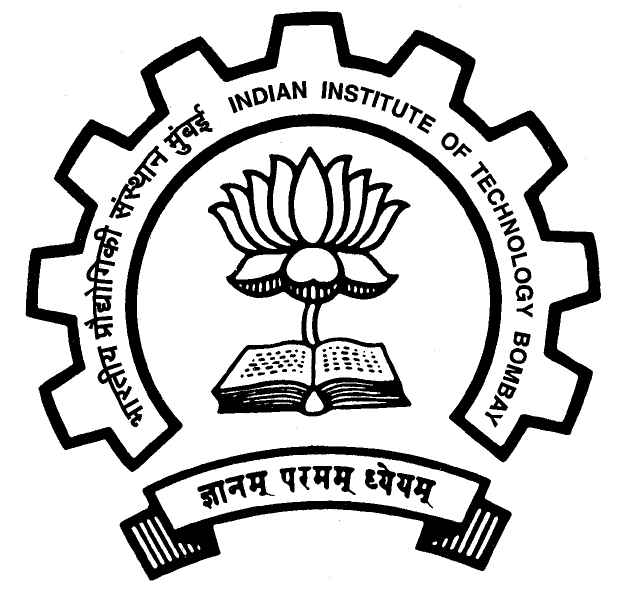
\includegraphics[scale=0.1]{logo.jpg}}\\
	\Large
	Inter-disciplinary program\\
	\Large
	in\\
	\Large
	Industrial Engineering and Operations Reserach (IEOR)\\
	\Large
	IIT BOMBAY\\
	\Large
		(2016-17)
\end{center}
\end{titlepage}
%\chapter*{Approval sheet}
%This is to certify that 
\chapter*{Declaration}
I declare that this written submission represents my idea in my own words and where others's idea or words have been included ,I have adequately cited and referenced the original source.I also declare that I have adhered to all principles of academic honesty and integrity and have not misrepresented or fabricated or falsified any/data/fact/source in my submission.I understand that any violation of the above will be cause for disciplinary action by the institute and can also evoke penal action from the sources which have thus not been properly cited or from whom proper permission has not been taken when needed.
\vspace{1cm}


\noindent Date:\hfill Prakash Arjun Gawas                     
\begin{flushright}(153190002)\end{flushright}
\chapter*{Acknowledment}
I would like to extend thanks to the many people who so generously contributed to the work presented in the thesis.Special mention goes to my enthusiastic supervisor, \textbf{Prof. Veeraruna Kavitha} for giving me opportunity of working under his guidence.His Direction, motivation,affectionate guidance and support have been the source of inspiration to bring the report this shape.I thank all the other faculty member of Industrial Engineering And Operations Research, who made me realize the virtue of learning through sustained hard work.
\vspace{6mm}

\noindent I would like to thanks all those whose name i missed but have contributed in any form for building up of the thesis upto now.
\vspace{1cm}

\begin{flushright}
Prakash Arjun Gawas\\
(153190002)
\end{flushright}

\chapter*{Abstract}
The project study is based on the
\tableofcontents
\listoffigures
\listoftables
\chapter{Preamble}
\section{Introduction}
Markov Decision process (MDP) is a mathematical framework that solves the problem of sequential decision making under uncertainty, to obtain an optimal policy. At each decision epoch the system state provides the decision maker with all necessary information for choosing an action from available actions in that state. As result of an action the decision maker receives a reward and the system state evolves to possibly different state at the next epoch depending on the controlled transition probability. Each action, the decision maker chooses in any particular state and at any time slot t, will have an associated reward/running cost $(R_t)$. The reward depends also on the current system state. In case of finite horizon problems, it also considers a terminal cost that only depends upon the state at termination. Hence over time the decision maker will receive a sequence reward/costs.\\

\noindent A policy is a sequence of such actions/rules, which the decision maker chooses at any time epoch depending on the state of the system. The aim of MDP is to find a policy prior to the first decision epoch that maximizes a function f of these reward sequences. In general MDP optimizes the expected value of the function f that defines a way of aggregating the running costs related to all the time slots under consideration, i.e., to optimize $E[f(R_1,R_2,...)]$. Linear MDPs consider expected value of either sum of all the running costs $E[\sum_t{R_t} ]$, or sum of discounted values of all the running costs $E[\sum_t{\beta^t {R_t}} ]$ with discount factor $\beta<1$ or time average of the running costs $\displaystyle\lim_{T \to \infty}\frac{[E[\sum_{t\leq T}{R_t}]}{T}$ .They are respectively called total cost, discounted cost or average cost problems. Also MDP problem can either be modelled over a finite time horizon or over the infinite time horizon. \\


\noindent Linear MDPs also called risk neutral MDPs control the first moment (expected value) of the sum cost. Optimization of the expected cost of an MDP is well studied. Many approaches have been developed to solve the problem. Dynamic programming (DP) is very popular technique to find optimal policies for finite horizon problems. Dynamic programming involves finding the optimal expected cost using Backward Induction. It basically solves a big problem by dividing it into many sub problems and than optimizing these sub problems. This is based on the famous Optimality equations from given in []. This gives rise to what is known as the Principle of Optimality where no matter what the current state and initial decision are, the remaining decisions must constitute an optimal policy with regard to the state resulting from the first decision. Others solution methods include Value and Policy iteration and its variants. These are iterative algorithms based on fixed point equations derived from the Optimality equations the theory of equations on normed linear spaces. The relationship between discounted MDPs and Linear programs (LPs) is also pretty well defined. Though not efficient LPs have elegant theory, ease in addition of additional constraints and facility of sensitivity analysis make it very attractable in some cases. LPs are derived based on Properties of the solutions to the optimality equations [citing theorem in puterman]. Primal linear program finds the optimal value while its dual gives the optimal policy to be followed.\\


In some situations we may also want to control the fluctuations around the expected value than we need to turn to Risk Sensitive MDPs (RSMDPs). RSMDPs can have varied applications in diverse fields. From investment of funds to manufacturing processes one can use RSMDPs to find optimal decisions. RSMDPs basically mean giving varied importance to higher moments of the total expected cost. One can also just optimize a function of mean and variance only as in [].  The literature on RSMDPs is relatively limited though. In [], Howard and Matheson have considered the maximisation of total reward with a constant risk sensitive parameter. They have discussed the application of iterative algorithms like Value Iteration and Policy Iteration to risk sensitive case. Recently in [] ,authors have proposed an LP based approach to solve the RSMDPs for finite horizon problem. Also they have augmented the state space appropriately so as to make addition of more constrains simple. The relation between LPs and infinite horizon is even more complex and needs to be investigated.\\ 


\noindent MDPs can be applied to varied examples in real life situations. One such application is the classic inventory control problem. In Inventory Control problem the decision maker must decide how much to order in each time period to meet demand for its products. The demand  is considered to be stochastic, where the distribution function is known. The objective here is to find a policy of ordering at any time epoch so as to minimize the total cost incurred for total period of time T thus making it a finite horizon problem. The various cost incurred depends on the current state of inventory, amount ordered and demand in that time period. There are three basic cost considered in this situation. Ordering cost that includes total  ordering cost of the quantity and also fixed order set-up cost. Holding cost for storing inventory and carrying it into the next period. Shortage cost is applicable when we cannot fulfil the demand on hand. All the costs are considered to be linear. Hence depending upon the demand the current inventory appropriate probability depending on the distribution. Thus this problem can be modelled using Markov chain. First we model it into a sequential decision model defining appropriate state space, actions, transition probability and rewards at each time epoch.  If we solve this problem using one of the techniques mentioned previously, the policy that the decision maker has to follow to optimize the expected reward only  is of the type (s,S). This means that whenever the inventory level goes below the level s will order so as to increase are inventory level to S, if not than we will not order. In [], Herbert Scarf has shown that when holding cost and shortage cost are linear then the optimal policy in each period is always of this type. The aim in my work is to find optimal policies for a risk averse decision maker. [] has given LP model for risk sensitive MDPS which can be applied for this example. \\

In [section 3] I have defined the model and the notations. The rewards pertaining to the linear MDP have been identified. There were two ways in which we could modelled the rewards for this problem. One way was that given the current state of the inventory and the action we can find the average reward at that point. Other was to shift the holding and shortage cost from the current period to the next period. Both the cases were solved using LP formulation given in [] and also by dynamic program and the results were validated. Furthermore in section 5 i present the model for risk sensitive MDPs.

\chapter{Literature Survey}


\noindent Classical MDPs deal with the maximisation of cumulative reward, however a decision maker may focus on several other distributional properties. Most decision makers maker may be risk averse i.e. they would like to reduce their risk and thus this forms the basis of a risk sensitive model. 
One way is to focus on mean and variance of the cumulative reward. Mean-variance optimisation has varied applications from finance to manufacturing fields.\\

In [], authors deal with various computational complexities of mean-variance optimisation. They show that these mDP are typically NP hard, but can admit pseudopolynomial algorithms.  The main problem with mean-variance optimisation is the absence of principle of optimality which could have led to simple recursive algorithms. This may give rise to situations where a decision maker can receive unexpected high rewards in the initial stages and may incur loss in the later stages to keep the variance small.  Also variance $ (Var(W))=E(W^2)- (E(W))^2$ is not a linear measure of the probability measure of the process. This is addressed using constrained Markov Decision Process to develop pseudo polynomial exact or approximate algorithms. They have defined their MDP model and compared different types of policies classes. The question they are addressing is that given a MDP M and rational numbers $\lambda$, $\nu$ does there exist a policy in the set $\prod$ such that $E(W)\geq \lambda$ and $Var(W)\leq \nu$. They  and established NP-hardness of this problem for all type of policies. Considering bounded integer rewards, they have identified cases for the existence of exact pseudo polynomial time algorithms. LP approach cannot be used directly used for the problem due to convexity issues in Mean Variance MDPs. Hence they augment the state space to exploit convexity to devise a pseudopolynomial algorithm.  Approximate algorithms are also given where they approximate mean and variance. On similar lines as previously they consider integer rewards the authors have proved existence of a polynomial time algorithm. For any general reward case we can discretize the rewards and obtain new MDP which will be equivalent to one with integer rewards and the same algorithm can be applied.\\

In [], authors apply risk sensitive approach to design plans for total productive maintenance (TPM). TPM  focuses on improving the overall effectiveness of a manufacturing facility by eliminating the waste of time and resources. Their aim was to find optimal productive maintenance (PM) time. PM help reduce the frequency of unexpected repairs when failure rate is of increasing nature. Traditional approaches in TPM only used expected value of the long run cost and overlooked the risk associated with the high cost. In actual practice risk sensitive managers would use the expected value of long-run cost and then use a factor of safety for the same optimal time. This is a heuristic approach and is more conservative. They give mean variance model where the objective function is $g(\tau)= \mu_C+ \theta {\sigma}^2$ with $\theta>0$, where $\mu_C$ and $\sigma^2$ denote the long-run mean and the long-run variance, respectively, of the net cost per unit time incurred from following a preventive maintenance plan that prescribes $\tau$ as the time for PM.An alternative formulation in terms of rewards, in which the objective function is maximized,is $g(\tau)= \mu_R- \theta {\sigma}^2$ with $\theta>0$, where $\mu_R$ and $\sigma^2$ denote the long-run mean and variance of the net reward per unit time, respectively. Risk neutral models have $\theta =0$. Typically $/theta$ is selected experimentally.TPM plans for the production line in its entirety tend to be
distinct from those for individual units that operate independently of the line. Hence they have developed separate models for the individual-unit scenario and the production-line scenario. For the case of the individual unit, a renewal-theory model is used. Here every failure or a maintenance triggers a so-called renewal event. Using Renewal Reward Theory he has derived an expression for $g(\tau)$ in terms of $\tau$, failure distribution and the individual cost of repair and maintenance. For the case of the production line a more involved model based on MDPs is used. He first develops the MDP identifies a Quadratic Program given in [] to solve the MDP. But solving the QP this is computationally expensive. He present an approach based on linearising the quadratic objective function by using a surrogate form for variance. Optimization could then be performed via linear programming. The existence of a deterministic policy is then proved for the surrogate objective function using DP approach to solve the problem by deriving the necessary optimality conditions. Using this he proposes a PI algorithm and shows its convergence. Computational results showed that the surrogate function did mimic the exact function reasonably well and also proves convergence in relatively short period of time.\\

In [], authors talk about risk sensitive planning with one switch utility functions. One switch utility functions model a decision maker whose decision change with their wealth level. For example a decision maker with low wealth levels may be risk averse, but may become risk neutral as the wealth level increases. These function model the risk attitude of decision maker.A decision maker is risk-neutral if their utility function is linear, risk-averse if their utility function is concave, and risk-seeking if their utility function is convex. Here one need to maximise the expected utility of a MDP for a given one switch utility function. This is difficult since the resulting planning problem is not decomposable. They model a probabilistic planning problem as a fully observable Goal-Directed Markov Decision Problems (GDMDPs) and investigate how to maximize the expected utility. The optimal course of action now depends not only on the current state of the GDMDP but also the wealth level. Thus the authors first gives an approach to transform the risk sensitive GDMDP (RS-GDMDP) into a risk neutral one by augmenting the state space of the RS-GDMDP with possible wealth levels. The authors than relate the values and policies of the original and augmented GDMDP.  The resulting RS-GDMDP has an infinite state space but its properties allow us to generalize the standard risk sensitive version of Value Iteration (VI) which manipulates to a risk sensitive version of VI, which manipulates the functions that map wealth level to values.\\

In [], the authors give varying importance to sample path trajectories and the expected value, as controlled by a parameter $\gamma$. Depending upon $\gamma$, called the risk parameter, it provides importance to higher moments of the sum cost. The aggregation function in this case equals the exponential of the sum of the running costs, $E[e^{-\gamma {\sum_{t\leq T}R_t}} ]$. Note that $E[e^{-\gamma {\sum_{t\leq T}R_t}} ]= E\frac{\sum_k ?^k {\sum_{t\leq T}{R_t}}^{k}}{k!}]$. While the linear MDPs control the ?rst moment (expected value) of the sum cost, the risk sensitive MDPs also control the variability/fluctuations around the expected value, by considering the higher moments. The linear MDPs are also viewed as risk neutral MDPs with $\gamma=0$. In this paper the authors provide connection between DP equations and two appropriate LPs for ?nite horizon case. The primal LP provides the value function while the dual LP provides the optimal policy. For LP?s in risk sensitive MDPs the authors have circumvented this problem by incorporating the multiplicative cost term into the mapping that converts any given Markov policy to a feasible point of the LP. This due to the fact that it is possible to construct the linear objective function of the relevant LP using the running costs of all time slots but the cost accumulates in a multiplicative manner for risk sensitive MDPs and hence the same approach cannot be adapted directly for constructing an LP for risk MDP. The authors also have discussed how to add more constraints to the LP by augmenting the state space with an extra component, which is representative of this multiplicative cost. They have also discussed two applications of the problem. First application includes delay tolerant networks where a message has to be transferred from a source to a faraway destination with the help of occasional contacts between the freely moving nodes (that are willing to become the relays) and the source/destination. Second application includes a lossy (finite buffer) queuing system with two server modes and with a constraint on the utilization of fast server mode. They have also compared the risk neutral policies with risk sensitive policies for the constrained MDP problem.\\

In [], Herbert Scarf considers a dynamic inventory problem where he considers ordering costs, holding costs and shortage costs. The underlying assumption here is that the holding and shortage cost are linear. He shows that when this is true the optimal policy in each period is always of the type (S,s). This means that whenever the inventory level goes below level s will order so as to increase are inventory level to S, if not than we will not order. He builds a total cost function, composed of the three costs described above. This function can be used to construct a dynamic program equation. He shoes the total cost function follows K-convexity. Due to this the optimal policy the optimal policy turns out to be of such simple form.\\

\chapter{Problem Description}
Consider an Inventory system that can be stocked to a maximum size of M. Let N be the number of planning horizons. A sequence of ordering decisions is made at the beginning of number of equally spaced intervals. The inventory builds upon ordering stock and depletes on fulfilling demand. Following assumptions apply to the model 
\begin{enumerate}
\item[\textbf{1)}] Demand $\xi$ are independent and identically distributed by a common distribution function f($\xi$).
\item[\textbf{2)}] All orders are placed at the start of the period and received immediately and lag is zero.
\item[\textbf{3)}] Demands arrive at the start of the period and are fulfilled instantly.
\item[\textbf{4)}] Holding and shortage costs are charged linearly.
\item[\textbf{5)}] Unsatisfied demand is lost forever.
\end{enumerate}
\noindent Now we define the different costs associated with the inventory process.\\
\begin{enumerate}
\item[\textbf{1)}] Order cost $(C_o)$ : This contains two components:
\begin{enumerate}
\item[\textbf{a)}] Fixed order cost (K) ? This the fixed cost for an order irrespective of the number of units you order.
\item[\textbf{b)}] Variable cost : This is a linear cost cost directly proportional to number of units you order.\\
\end{enumerate}
\begin{equation*}
C_o = 
\begin{cases}
0   \hspace{2.12cm}          ,a&=0\\
K+ c_u {a}     \hspace{1cm}           ,a&>0
\end{cases}
\end{equation*}

\hspace{6mm} Where 'a' is the amount of quantity ordered and $c_u$  is the unit price

\item[\textbf{2)}]Holding cost $(C_H)$ : Cost associated with storing the inventory that remain unsold. This cost will depend on the demand.

\begin{equation*}
C_H = 
\begin{cases}
0   &,\xi \geq s+a\\
c_H(s+a-\xi)     & ,\xi <s+a
\end{cases}
\end{equation*}
\begin{flushleft}Where $c_k$ is the unit holding cost.
\end{flushleft}

\item[\textbf{3)}]	Shortage cost$(C_S)$ : Cost associate with not being able to fulfil demand from the stock. 

\begin{equation*}
C_S = 
\begin{cases}
0          &,\xi \leq s+a\\
C_S(\xi-s-a)     &  ,\xi >s+a
\end{cases}
\end{equation*}
\begin{flushleft}where $c_s$ is the unit shortage cost.
\end{flushleft}
\end{enumerate}
A Markov decision process formulation follows below:\\
\noindent Decision Epochs:\\
\begin{equation*}T = \lbrace 1,2,3,...N \rbrace,   N \leq \infty. 
\end{equation*}\\
\noindent State space:\\
\begin{equation*}S = \lbrace 0,1,2,...M \rbrace  
\end{equation*}\\
\noindent Actions:\\
\begin{equation*}A_s  = \lbrace0,1,2,...M-s \rbrace
\end{equation*}\\
\noindent Expected Rewards:\\
\begin{equation*}r_t(s,a) = (c_o+c_H+c_s) 
\end{equation*}


\begin{equation*}
p(j|s,a)=
\begin{cases}
f(\xi\cong s+a-j)&,{s+a}>j\geq0\\
f(\xi\geq s+a)&,j=0\\
0&,\text{else}
\end{cases}
\end{equation*}

\end{document}
